\newif\ifglobal

%%%%%%%%%%%%%%%%%%%%%%%
%%% Compile to view %%%
%%%%%%%%%%%%%%%%%%%%%%%

%%%%%%%%%%%%%%%%%%%%%%%%%%%%%%%%%%%%%%%%%%%%%%%%%%%
%%% Readme:                                     %%%
%%% https://www.overleaf.com/read/bwdjvfjksvjy/ %%%
%%%%%%%%%%%%%%%%%%%%%%%%%%%%%%%%%%%%%%%%%%%%%%%%%%%

% >>> M?: marks a module setting number or important notice

% >>> M4: Set {./relative-path} to external files for this module <<<
\def \modulefiles {./29-HMAC}
% To add an external file, use:
% (Replace '---' with actual filename)
% '\input{\modulefiles/tables/---.tex}' for tables
% '\includegraphics{\modulefiles/figures/---}' for figures
% '\subfile{\modulefiles/---}' for register files

% >>> M1: This module is in global project? <<<
% 'YES' - uncomment; 'NO' - comment out
\globaltrue

\ifglobal
    \documentclass[main\_\_EN.tex]{subfiles}

\else
    \documentclass[openany, 10pt]{book}

    % >>> M2: In ./00-shared/preamble-trm-module, also find
    %         settings for visibility of todo notes, watermark <<<
    \usepackage{preamble-trm-module}

    % >>> M3: Temporary labels in English,
    %         you can add your own labels there <<<
    \myexternaldocument{./00-shared/temp-labels-en}

\fi %\ifglobal


\setcounter{secnumdepth}{4}

% >>> M5: If this module needs any updates in
% './00-shared/preamble-trm-module.sty'
% (include additional package, etc.), contact your module PM
% or create the file './00-shared/changelog.tex' make the
% necessary updates yourself and document them in this file <<<


\begin{document}


% Sets language into which pre-defined bits of text are translated
\selectlanguage{english}

% Do not delete this block
\ifglobal
% Add the following front matter if
% this module is outside of global project
\else
    \InputIfFileExists{readme}{}{}
    {\let\clearpage\relax \listoftodos}
    \tableofcontents
    %\listoftables
    %\listoffigures
\fi


%%%%%%%%%%%%%%%%%%%%%%%%%
%%% TRM Module Begins %%%
%%%%%%%%%%%%%%%%%%%%%%%%%


\hypertarget{hmac}{}
\chapter{HMAC Accelerator (HMAC)}
\label{mod:hmac}


The Hash-based Message Authentication Code (HMAC) module computes Message Authentication Codes (MACs) using Hash algorithm and keys as described in RFC 2104. The underlying hash algorithm is SHA-256, and the 256-bit HMAC key is stored in an eFuse key block and can be set as read-protected for users.

\section{Main Features}
\begin{itemize}
    \item Standard HMAC-SHA-256 algorithm
    \item Hash result only accessible by configurable hardware peripheral (in downstream mode)
    \item Compatible to challenge-response authentication algorithm
    \item Generates required keys for RSA\_DS (in downstream mode)
    \item Re-enables soft-disabled JTAG (in downstream mode)
\end{itemize}

\section{Functional Description}

The HMAC module operates in two modes: upstream mode and downstream mode. In upstream mode, the HMAC message is provided by the user and the calculation result is read back by the user; in downstream mode, the HMAC module is used as a Key Derivation Function (KDF) for other internal hardware. For instance, the JTAG can be temporarily disabled by burning odd number bits of \hyperref[fielddesc:EFUSESOFTDISJTAG]{EFUSE\_SOFT\_DIS\_JTAG} in eFuse. In this case, users can temporarily re-enable JTAG using the HMAC module in downstream mode.

After the reset signal being released, the HMAC module will check whether the RSA\_DS\_KEY exists in the eFuse. If the key exists, the HMAC module will enter downstream RSA\_DS mode and finish the RSA\_DS\_KEY calculation automatically.

\subsection{Upstream Mode}

Common use cases for the upstream mode are challenge-response protocols supporting HMAC-SHA-256 algorithm. In upstream mode, the user should provide the related HMAC information and read back its calculation results.

Assume the two entities in the challenge-response protocol are A and B respectively, and the entities share the same secret KEY. The data message they expect to exchange is M. The general process of this protocol is as follows:

\begin{itemize}
    \item A calculates a unique random number M
    \item A sends M to B
    \item B calculates the HMAC value (through M and KEY) and sends the result to A
    \item A also calculates the HMAC value (through M and KEY) internally
    \item A compares these two values. If they are the same, then the identity of B is authenticated
\end{itemize}

To calculate the HMAC value (the following steps should be done by the user):

\begin{enumerate}
    \item Initialize the HMAC module, and enter upstream mode.
    \item Write the correctly padded message to the HMAC, one block at a time.
    \item Read back the result from HMAC.
\end{enumerate}

For details of this process, please see Section \ref{sec:hmac-process-detailed}.

\subsection{Downstream JTAG Enable Mode}

There are two parameters in the eFuse memory to disable JTAG debugging, namely \hyperref[fielddesc:EFUSEDISPADJTAG]{EFUSE\_DIS\_PAD\_JTAG} and \hyperref[fielddesc:EFUSESOFTDISJTAG]{EFUSE\_SOFT\_DIS\_JTAG}. Set \hyperref[fielddesc:EFUSEDISPADJTAG]{EFUSE\_DIS\_PAD\_JTAG} to 1 can disable JTAG permanently, and set odd numbers of 1 to \hyperref[fielddesc:EFUSESOFTDISJTAG]{EFUSE\_SOFT\_DIS\_JTAG} can disable JTAG temporarily. For more details, please see Chapter \ref{mod:efuse} \textit{\nameref{mod:efuse}}.

To re-enable the temporarily disabled JTAG, users can follow the steps below:

\begin{enumerate}
\item Enable the HMAC module and enter downstream JTAG enable mode.
\item Write 1 to the \hyperref[regdesc:HMACSOFTJTAGCTRLREG]{HMAC\_SOFT\_JTAG\_CTRL\_REG} register to enter JTAG re-enable compare mode.
\item Write the 256-bit HMAC value which is calculated locally from the 32-byte 0x{}00 using HMAC-SHA-256 algorithm and the pre-generated key to register \hyperref[regdesc:HMACWRJTAGREG]{HMAC\_WR\_JTAG\_REG}, in big-endian order of word.
\item If the HMAC internally calculated value matches the value that user programmed, then JTAG is re-enabled. Otherwise, JTAG remains disabled.
\item JTAG remains in the status as in step 4 until the user writes 1 to register \hyperref[regdesc:HMACSETINVALIDATEJTAGREG]{HMAC\_SET\_INVALIDATE\_JTAG\_REG} or restart JTAG.
\end{enumerate}

For detailed steps of this process, please see Section \ref{sec:hmac-process-detailed}.

\subsection{Downstream RSA\_DS Mode}

The RSA Digital Signature Peripheral (RSA\_DS) encrypts its parameters using AES-CBC algorithm. The HMAC module is used as a Key Derivation Function (KDF) to derive the AES key to decrypt these parameters.

Before starting the RSA\_DS peripheral, the user needs to obtain the key for it first through HMAC calculation. For more information, please see Chapter \ref{mod:digsig} \textit{\nameref{mod:digsig}}. After the clock of HMAC be enabled and reset of HMAC be released, the HMAC module will check to see if there is a functional key in eFuses for the RSA\_DS peripheral. If yes, HMAC will enter downstream RSA\_DS mode and finish RSA\_DS\_KEY calculation automatically.

\subsection{HMAC eFuse Configuration}
\label{sec:hmac-config-function}

The HMAC module provides three different functionalities: re-enabling JTAG and serving as RSA\_DS KDF in downstream mode as well as pure HMAC calculation in upstream mode. Table \ref{tab:hmac-key-purpose} lists the register value corresponding to each purpose, which should be written to register \hyperref[regdesc:HMACSETPARAPURPOSEREG]{HMAC\_SET\_PARA\_PURPOSE\_REG} by the user (see Section \ref{sec:hmac-process-detailed}).

\clearpage
\input{./29-HMAC/tables/29-HMAC-key-purpose__EN}

Before enabling HMAC to do calculations, user should make sure the key to be used has been burned in eFuse. You can burn a key to eFuse as follows:

\begin{enumerate}
    \item Prepare a secret 256-bit HMAC key and burn the key to an empty eFuse block $y$ (there are six blocks for storing a key in eFuse. The numbers of those blocks range from 4 to 9, so $y$ = 4,5,..,9. Hence, if we are talking about key0, we mean eFuse block4), and then program the purpose to EFUSE\_KEY\_PURPOSE\_$(y-4)$. Take upstream mode as an example: after programming the key, the user should program EFUSE\_KEY\_PURPOSE\_HMAC\_UP (corresponding value is 8) to EFUSE\_KEY\_PURPOSE\_$(y-4)$. Please see Chapter \ref{mod:efuse} \textit{\nameref{mod:efuse}} on how to program eFuse keys.
    \item Configure this eFuse key block to be read protected, so that users cannot read its value. A copy of this key should be kept by any party who needs to verify this device.
\end{enumerate}

\subsection{HMAC Initialization}

The eFuse key blocks (with correctly programmed purpose values) must be coordinated with the HMAC modes, or HMAC will terminate calculation.

\textbf{Configure HMAC modes}

The correct purpose (see Table \ref{tab:hmac-key-purpose}) has to be written to register \hyperref[regdesc:HMACSETPARAPURPOSEREG]{HMAC\_SET\_PARA\_PURPOSE\_REG} by the user.

\textbf{Select eFuse Key Blocks}
\label{sec:hmac-config-efuse-key}

The eFuse controller provides six key blocks, i.e., KEY0 \verb+~+ 5. To select a particular KEY\textcolor{red}{n} for a certain HMAC calculation, write the key number \textcolor{red}{n} to register \hyperref[regdesc:HMACSETPARAKEYREG]{HMAC\_SET\_PARA\_KEY\_REG}.

Note that the purpose of the key has also been programmed to eFuse memory. Only when the configured HMAC purpose matches the defined purpose of KEY\textcolor{red}{n}, will the HMAC module execute the configured calculation. Otherwise, it will return a matching error and stop the current calculation.
For example, suppose a user selects KEY3 for HMAC calculation, and the value programmed to KEY\_PURPOSE\_3 is 6 (EFUSE\_KEY\_PURPOSE\_HMAC\_DOWN\_JTAG). Based on Table \ref{tab:hmac-key-purpose}, KEY3 can be used to re-enable JTAG. If the value written to register \hyperref[regdesc:HMACSETPARAPURPOSEREG]{HMAC\_SET\_PARA\_PURPOSE\_REG} is also 6, then the HMAC module will start the process to re-enable JTAG.


\subsection{HMAC Process (Detailed)}
\label{sec:hmac-process-detailed}

The process to call HMAC in \chipname{} is as follows:

\begin{enumerate}
    \item Enable HMAC module
    \begin{enumerate}
        \item Set the peripheral clock bits for HMAC and SHA peripherals in SYSTEM\_PEIRP\_CLK\_EN1\_REG, and clear the corresponding peripheral reset bits in SYSTEM\_PEIRP\_RST\_EN1\_REG. For registers information, please see Chapter \ref{mod:sysmem} \textit{\nameref{mod:sysmem}}.
        \item Write 1 to register \hyperref[regdesc:HMACSETSTARTREG]{HMAC\_SET\_START\_REG}.
    \end{enumerate}

    \item Configure HMAC keys and key purposes
    \begin{enumerate}
        \item Write the key purpose $m$ to register \hyperref[regdesc:HMACSETPARAPURPOSEREG]{HMAC\_SET\_PARA\_PURPOSE\_REG}. The possible key purpose values are shown in Table \ref{tab:hmac-key-purpose}. For more information, please refer to Section \ref{sec:hmac-config-function}.
        \item Select KEY\textcolor{red}{n} in eFuse memory as the key by writing \textcolor{red}{n} (0 \verb+~+ 5) to register \hyperref[regdesc:HMACSETPARAKEYREG]{HMAC\_SET\_PARA\_KEY\_REG}. For more information, please refer to Section \ref{sec:hmac-config-efuse-key}.
        \item Write 1 to register \hyperref[regdesc:HMACSETPARAFINISHREG]{HMAC\_SET\_PARA\_FINISH\_REG} to complete the configuration.
        \item Read register \hyperref[regdesc:HMACQUERYERRORREG]{HMAC\_QUERY\_ERROR\_REG}. If its value is 1, it means the purpose of the selected block does not match the configured key purpose and the calculation will not proceed. If its value is 0, it means the purpose of the selected block matches the configured key purpose, and then the calculation can proceed.
        \item When the value of \hyperref[regdesc:HMACSETPARAPURPOSEREG]{HMAC\_SET\_PARA\_PURPOSE\_REG} is not 8, it means the HMAC module is in downstream mode, proceed with Step 3. When the value is 8, it means the HMAC module is in upstream mode, proceed with Step 4.
    \end{enumerate}

    \item Downstream mode
    \begin{enumerate}
        \item Poll Status register \hyperref[regdesc:HMACQUERYBUSYREG]{HMAC\_QUERY\_BUSY\_REG}. When the value of this register is 0, HMAC calculation in downstream mode is completed.
        \item In downstream mode, the calculation result is used by either the JTAG or RSA\_DS peripheral in the hardware.
        To clear the result and make further usage of the dependent hardware (JTAG or RSA\_DS), write 1 to either register \hyperref[regdesc:HMACSETINVALIDATEJTAGREG]{HMAC\_SET\_INVALIDATE\_JTAG\_REG} to clear the result generated by JTAG key; or to register \hyperref[regdesc:HMACSETINVALIDATEDSREG]{HMAC\_SET\_INVALIDATE\_DS\_REG} to clear the result generated by RSA\_DS\_KEY.
        \item Downstream mode operation completed.
    \end{enumerate}

    \item Transmit message block Block\_\textcolor{red}{n} ($\textcolor{red}{n}>=1$) in upstream mode
    \begin{enumerate}
        \item Poll Status register \hyperref[regdesc:HMACQUERYBUSYREG]{HMAC\_QUERY\_BUSY\_REG}. When the value of this register is 0, go to step 4(b).
        \item Write the 512-bit Block\_\textcolor{red}{n} to register \\HMAC\_WDATA0\verb+~+15\_REG. Write 1 to register \hyperref[regdesc:HMACSETMESSAGEONEREG]{HMAC\_SET\_MESSAGE\_ONE\_REG}, to trigger the processing of this message block.
        \item Poll Status register \hyperref[regdesc:HMACQUERYBUSYREG]{HMAC\_QUERY\_BUSY\_REG}. When the value of this register is 0, go to step 4(d).
        \item Different message blocks will be generated, depending on whether the size of the to-be-processed message is a multiple of 512 bits.
        \begin{itemize}
            \item If the bit length of the message is a multiple of 512 bits, there are three possible options:
            \begin{enumerate}
                \item If Block\_\textcolor{red}{n+1} exists, write 1 to register \hyperref[regdesc:HMACSETMESSAGEINGREG]{HMAC\_SET\_MESSAGE\_ING\_REG} to make $n=n+1$, and then jump to step 4(b).
                \item If Block\_\textcolor{red}{n} is the last block of the message and the user wants to apply SHA padding in hardware, write 1 to register \hyperref[regdesc:HMACSETMESSAGEENDREG]{HMAC\_SET\_MESSAGE\_END\_REG}, and then jump to step 6.
                \item If Block\_\textcolor{red}{n} is the last block of the padded message and the user has applied SHA padding in software, write 1 to register \hyperref[regdesc:HMACSETMESSAGEPADREG]{HMAC\_SET\_MESSAGE\_PAD\_REG}, and then jump to step 5.
            \end{enumerate}
            \item If the bit length of the message is not a multiple of 512 bits, there are three possible options as follows. Note that in this case, the user should apply SHA padding to the message, after which the padded message length should be a multiple of 512 bits.
            \begin{enumerate}
                \item If Block\_\textcolor{red}{n} is the only message block, \begin{math}n=1\end{math}, and Block\_\textcolor{red}{1} has included all padding bits, write 1 to register \hyperref[regdesc:HMACONEBLOCKREG]{HMAC\_ONE\_BLOCK\_REG}, and then jump to step 6.
                \item If Block\_\textcolor{red}{n} is the second to last padded block, write 1 to register\\ \hyperref[regdesc:HMACSETMESSAGEPADREG]{HMAC\_SET\_MESSAGE\_PAD\_REG}, and then jump to step 5.
                \item If Block\_\textcolor{red}{n} is neither the last nor the second to last message block, write 1 to register \\\hyperref[regdesc:HMACSETMESSAGEINGREG]{HMAC\_SET\_MESSAGE\_ING\_REG} and define $n=n+1$, and then jump to step 4.(b).
            \end{enumerate}
        \end{itemize}
    \end{enumerate}

    \item Apply SHA padding to message
    \begin{enumerate}
        \item After applying SHA padding to the last message block as described in Section \ref{sec:hmac-padding}, write this block to register HMAC\_WDATA0\verb+~+15\_REG, and then write 1 to register \hyperref[regdesc:HMACSETMESSAGEONEREG]{HMAC\_SET\_MESSAGE\_ONE\_REG}. Then the HMAC module will calculate this message block.
        \item Jump to step 6.
    \end{enumerate}

    \item Read hash result in upstream mode
    \begin{enumerate}
        \item Poll Status register \hyperref[regdesc:HMACQUERYBUSYREG]{HMAC\_QUERY\_BUSY\_REG}. When the value of this register is 0, go to the next step.
        \item Read hash result from register HMAC\_RDATA0\verb+~+7\_REG.
        \item Write 1 to register \hyperref[regdesc:HMACSETRESULTFINISHREG]{HMAC\_SET\_RESULT\_FINISH\_REG} to finish calculation.
        \item Upstream mode operation is completed.
    \end{enumerate}

\end{enumerate}

\begin{tiplisting}
    The SHA accelerator can be called directly, or used internally by the RSA\_DS peripheral and the HMAC module. However, they can not share the hardware resources simultaneously. Therefore, SHA module can not be called by the CPU nor RSA\_DS peripheral when the HMAC module is in use.
\end{tiplisting}

\section{HMAC Algorithm Details}

\subsection{Padding Bits}
\label{sec:hmac-padding}
The HMAC module uses SHA-256 as hash algorithm. If the input message is not a multiple of 512 bits, a SHA-256 padding algorithm must be applied in software. The SHA-256 padding algorithm is the same as described in Section \emph{Padding the Message} of \emph{FIPS PUB 180-4}.

As shown in Figure \ref{fig:hmac-padding}, suppose the length of the unpadded message is $m$ bits. Padding steps are as follows:

\begin{enumerate}
    \item Append one bit of value ``1" to the end of the unpadded message;
    \item Append $k$ bits of value ``0", where k is the smallest non-negative number which satisfies $m + 1 + k {\equiv} 448 (mod 512)$;
    \item Append a 64-bit integer value as a binary block. This block includes the length of the unpadded message as a big-endian binary integer value $m$.
\end{enumerate}

\begin{figure}[ht!]
    \centering
    \fbox{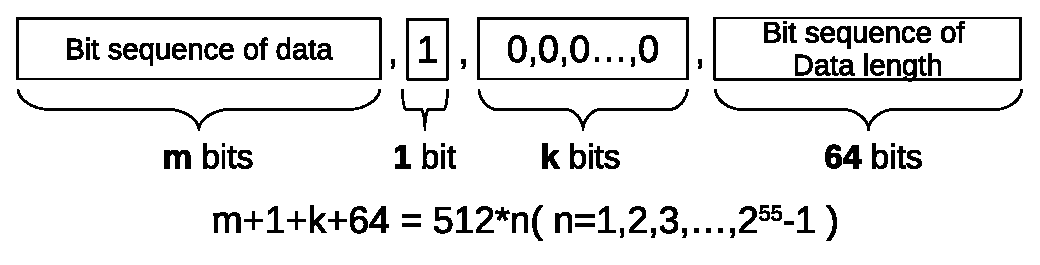
\includegraphics[width=0.7\textwidth]{./29-HMAC/figures/29-hmac-padding__EN}}
    \caption{HMAC SHA-256 Padding Diagram}
    \label{fig:hmac-padding}
\end{figure}

In downstream mode, there is no need to input any message or apply padding.
In upstream mode, if the length of the unpadded message is a multiple of 512 bits, the user can choose to configure hardware to apply the SHA padding. If the length is not a multiple of 512 bits, the user must apply the SHA padding manually. For detailed steps, please see Section \ref{sec:hmac-process-detailed}.

\subsection{HMAC Algorithm Structure}
The structure of the implemented algorithm in the HMAC module is shown in Figure \ref{fig:hmac-structure}. This is the standard HMAC algorithm as described in RFC 2104.

\begin{figure}[ht!]
    \centering
    \fbox{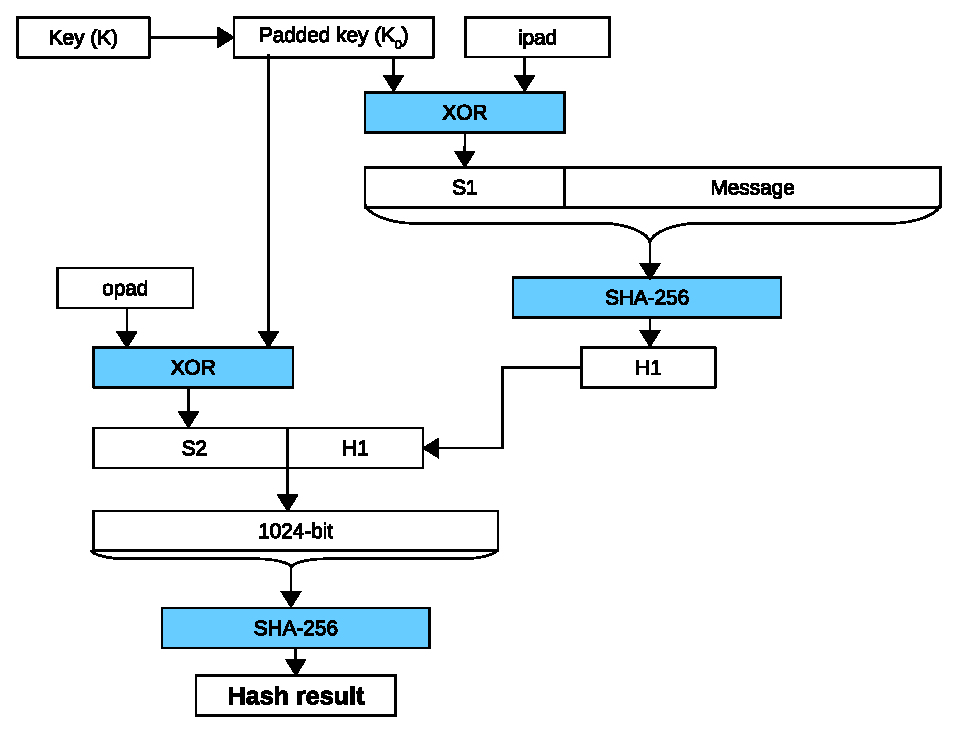
\includegraphics[width=0.65\textwidth]{./29-HMAC/figures/29-hmac-structure}}
    \caption{HMAC Structure Schematic Diagram}
    \label{fig:hmac-structure}
\end{figure}

\clearpage
In Figure \ref{fig:hmac-structure}:
\begin{enumerate}
    \item ipad is a 512-bit message block composed of 64 bytes of 0x{}36.
    \item opad is a 512-bit message block composed of 64 bytes of 0x{}5c.
\end{enumerate}

The HMAC module appends a 256-bit 0 sequence after the bit sequence of the 256-bit key K in order to get a 512-bit K$_0$. Then, the HMAC module XORs K$_0$ with ipad to get the 512-bit S1. Afterwards, the HMAC module appends the input message (multiple of 512 bits) after the 512-bit S1, and exercises the SHA-256 algorithm to get the 256-bit H1.

The HMAC module appends the 256-bit SHA-256 hash result H1 to the 512-bit S2 value, which is calculated using the XOR operation of K$_0$ and opad. A 768-bit sequence will be generated. Then, the HMAC module uses the SHA padding algorithm described in Section \ref{sec:hmac-padding} to pad the 768-bit sequence to a 1024-bit sequence, and applies the SHA-256 algorithm to get the final hash result (256-bit).

% >>> If your module has no registers, delete sample text
%       for Sections Register Summary and Registers below <<<

%%%%%%%%%%%%%%%%%%%%%%%%
%%% Register Summary %%%
%%%%%%%%%%%%%%%%%%%%%%%%

% >>> Update the sample text below and insert
%     the info on register summary into the subfile <<<

\clearpage
\hypertarget{hmac-reg-summ}{}
\section{Register Summary}
\label{sec:hmac-reg-summ}

The addresses in this section are relative to HMAC Accelerator base address provided in Table \ref{tab:sysmem-base-address} in Chapter \ref{mod:sysmem} \textit{\nameref{mod:sysmem}}.

The abbreviations given in Column \textbf{Access} are explained in Section \hyperref[glossary-access-types]{\textit{Access Types for Registers}}.

\subfile{\modulefiles/29-HMAC-reg-summ__EN}


%%%%%%%%%%%%%%%%%
%%% Registers %%%
%%%%%%%%%%%%%%%%%

% >>> Update the sample text below and insert
%      the info on registers into the subfile <<<

\clearpage
\section{Registers}

The addresses in this section are relative to HMAC Accelerator base address provided in Table \ref{tab:sysmem-base-address} in Chapter \ref{mod:sysmem} \textit{\nameref{mod:sysmem}}.

\subfile{\modulefiles/29-HMAC-reg__EN}


\end{document}
